\documentclass[letterpaper]{report}
%\usepackage[utf8]{inputenc}
\usepackage[T1]{fontenc}
\usepackage{RJournal}
\usepackage{amsmath,amssymb,array}
\usepackage{booktabs}

%% load any required packages here

\usepackage[spanish]{babel}
\usepackage{graphicx}

\hypersetup{pdftitle={mapeAr: aplicación interactiva para visualizar
información geográfica del turismo},
            pdfkeywords={Estadísticas
Públicas; Turismo; Argentina; Shiny; dataviz}}


\hypersetup{pdfauthor={Elián Soutullo, Juan Pablo Ruiz Nicolini}}

\newlength{\cslhangindent}
\setlength{\cslhangindent}{1.5em}
\newenvironment{CSLReferences}%
{\setlength{\parindent}{0pt}%
\everypar{\setlength{\hangindent}{\cslhangindent}}\ignorespaces}%
{\par}

%\usepackage[hidelinks]{hyperref}

\urlstyle{same}  % don't use monospace font for urls
\usepackage{color}
\usepackage{fancyvrb}
\newcommand{\VerbBar}{|}
\newcommand{\VERB}{\Verb[commandchars=\\\{\}]}
\DefineVerbatimEnvironment{Highlighting}{Verbatim}{commandchars=\\\{\}} 
% Add ',fontsize=\small' for more characters per line
\usepackage{framed}
\definecolor{shadecolor}{RGB}{248,248,248}
\newenvironment{Shaded}{\begin{snugshade}}{\end{snugshade}}
\newcommand{\AlertTok}[1]{\textcolor[rgb]{0.94,0.16,0.16}{#1}}
\newcommand{\AnnotationTok}[1]{\textcolor[rgb]{0.56,0.35,0.01}{\textbf{\textit{#1}}}}
\newcommand{\AttributeTok}[1]{\textcolor[rgb]{0.77,0.63,0.00}{#1}}
\newcommand{\BaseNTok}[1]{\textcolor[rgb]{0.00,0.00,0.81}{#1}}
\newcommand{\BuiltInTok}[1]{#1}
\newcommand{\CharTok}[1]{\textcolor[rgb]{0.31,0.60,0.02}{#1}}
\newcommand{\CommentTok}[1]{\textcolor[rgb]{0.56,0.35,0.01}{\textit{#1}}}
\newcommand{\CommentVarTok}[1]{\textcolor[rgb]{0.56,0.35,0.01}{\textbf{\textit{#1}}}}
\newcommand{\ConstantTok}[1]{\textcolor[rgb]{0.00,0.00,0.00}{#1}}
\newcommand{\ControlFlowTok}[1]{\textcolor[rgb]{0.13,0.29,0.53}{\textbf{#1}}}
\newcommand{\DataTypeTok}[1]{\textcolor[rgb]{0.13,0.29,0.53}{#1}}
\newcommand{\DecValTok}[1]{\textcolor[rgb]{0.00,0.00,0.81}{#1}}
\newcommand{\DocumentationTok}[1]{\textcolor[rgb]{0.56,0.35,0.01}{\textbf{\textit{#1}}}}
\newcommand{\ErrorTok}[1]{\textcolor[rgb]{0.64,0.00,0.00}{\textbf{#1}}}
\newcommand{\ExtensionTok}[1]{#1}
\newcommand{\FloatTok}[1]{\textcolor[rgb]{0.00,0.00,0.81}{#1}}
\newcommand{\FunctionTok}[1]{\textcolor[rgb]{0.00,0.00,0.00}{#1}}
\newcommand{\ImportTok}[1]{#1}
\newcommand{\InformationTok}[1]{\textcolor[rgb]{0.56,0.35,0.01}{\textbf{\textit{#1}}}}
\newcommand{\KeywordTok}[1]{\textcolor[rgb]{0.13,0.29,0.53}{\textbf{#1}}}
\newcommand{\NormalTok}[1]{#1}
\newcommand{\OperatorTok}[1]{\textcolor[rgb]{0.81,0.36,0.00}{\textbf{#1}}}
\newcommand{\OtherTok}[1]{\textcolor[rgb]{0.56,0.35,0.01}{#1}}
\newcommand{\PreprocessorTok}[1]{\textcolor[rgb]{0.56,0.35,0.01}{\textit{#1}}}
\newcommand{\RegionMarkerTok}[1]{#1}
\newcommand{\SpecialCharTok}[1]{\textcolor[rgb]{0.00,0.00,0.00}{#1}}
\newcommand{\SpecialStringTok}[1]{\textcolor[rgb]{0.31,0.60,0.02}{#1}}
\newcommand{\StringTok}[1]{\textcolor[rgb]{0.31,0.60,0.02}{#1}}
\newcommand{\VariableTok}[1]{\textcolor[rgb]{0.00,0.00,0.00}{#1}}
\newcommand{\VerbatimStringTok}[1]{\textcolor[rgb]{0.31,0.60,0.02}{#1}}
\newcommand{\WarningTok}[1]{\textcolor[rgb]{0.56,0.35,0.01}{\textbf{\textit{#1}}}}

\providecommand{\keywords}[1]{\noindent\textbf{Palabras clave:} #1}
\providecommand{\tightlist}{%
\setlength{\itemsep}{0pt}\setlength{\parskip}{0pt}}



\begin{document}

%% do not edit, for illustration only
\sectionhead{mapeAr: aplicación interactiva para visualizar información
geográfica del turismo}
\year{2021}

\begin{article}

\title{mapeAr: aplicación interactiva para visualizar información
geográfica del turismo}

\author{
Elián Soutullo , 
Juan Pablo Ruiz Nicolini }


\maketitle

\abstract{
Desarrollo de una shiny app que sirva como herramienta interactiva para
la visualización de mapas con información georeferenciada del turismo en
Argentina.
}

\keywords{ Estadísticas
Públicas  -  Turismo  -  Argentina  -  Shiny  -  dataviz }

\hypertarget{introducciuxf3n}{%
\subsection{Introducción}\label{introducciuxf3n}}

La visualización de datos es un recurso útil a la hora de comunicar y
pensar estrategias de desarrollo. En materia de política turística, como
en muchas otras áreas de la administración pública, trabajar con datos
geográficos resulta de vital importancia para la planificación y
promoción.

¿Dónde se localizan los principales atractivos turísticos de una
provincia? ¿Cuál es el nivel de concentración geográfica de los destinos
turísticos de un país? ¿Cómo se conectan las principales ciudades
receptoras de turismo? Este tipo de preguntas puede ser respondida de
manera gráfica y sencilla a través de la confección de mapas.

Sin embargo, la realización de un mapa que permita visualizar
información geográfica resulta ser una tarea un tanto compleja, en
especial si no se cuenta con conocimientos técnicos sobre
\textbf{Sistemas de Información Geográfica (SIG)}.

En este sentido, contar con una herramienta de acceso libre para la
representación de datos espaciales sin requerimientos de programación o
diseño, supone una solución para diversos usuarios interesados en el
tema.

El paquete \CRANpkg{shiny} (Chang et al. 2021) ofrece una oportunidad
para un desarrollo de estas características, al permitir construir una
aplicación con una interfaz accesible
\textbf{(\href{https://github.com/dnme-minturdep/mapeAr/blob/main/ui.R}{UI})}
y un trasfondo donde se procese la información geográfica
\textbf{(\href{https://github.com/dnme-minturdep/mapeAr/blob/main/server.R}{server})}.

\hypertarget{mapear}{%
\subsection{mapeAr}\label{mapear}}

\href{https://tableros.yvera.tur.ar/mapeAr/}{\textbf{mapeAr}} surge en
este contexto como un recurso de la Dirección Nacional de Mercados y
Estadística (DNMyE) en el marco del
\href{https://www.yvera.tur.ar/sinta/}{\textbf{Sistema de Información
Turística de la Argentina (SINTA)}}. La plataforma consiste de dos
pestañas, una con información sobre cómo utilizar la aplicación y otra
con los controles y visualización para poder realizar un mapa.

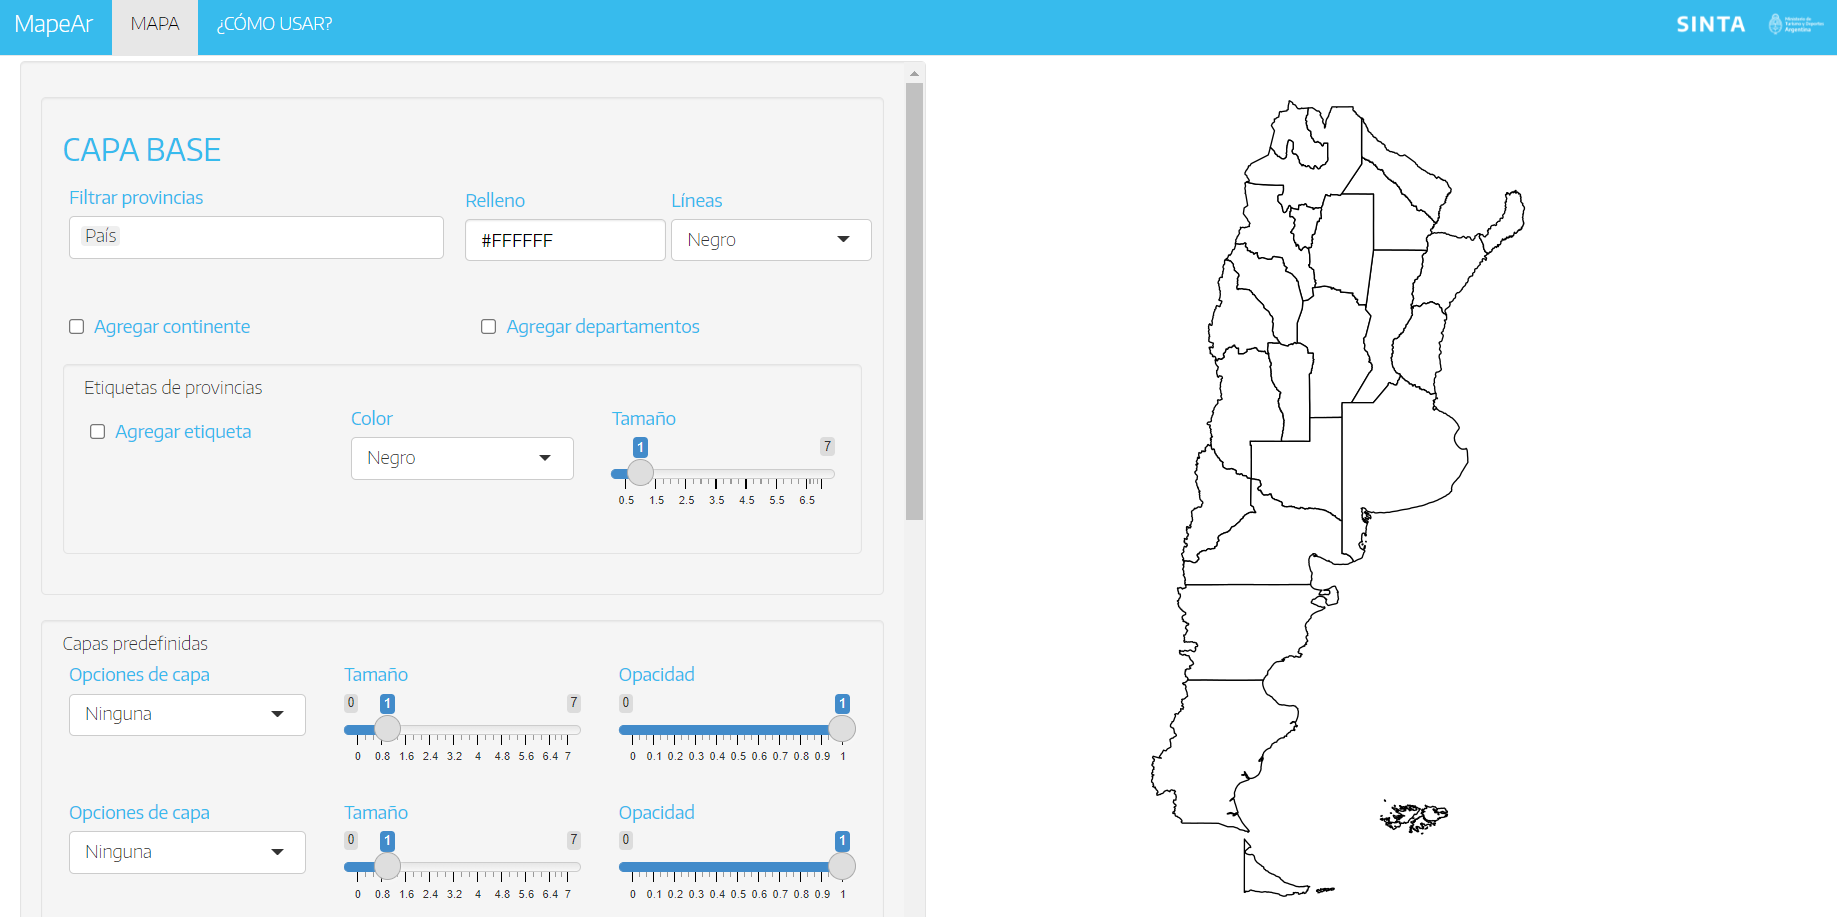
\includegraphics[width=0.8\linewidth,height=0.3\textheight]{imagenes/mapear}

Por defecto la \emph{shiny} carga una capa con la geometría de Argentina
y su división política (provincias). Esta es la denominada \textbf{capa
base}, sobre la cual se pueden hacer algunas modificaciones (filtrar
provincias específicas, agregar las etiquetas con los nombres, o los
polígonos correspondientes a la región, por ejemplo).

Utilizando la lógica de \CRANpkg{ggplot2} (Wickham 2016), la aplicación
permite incorporar más capas de datos georeferenciados sobre la capa
base. En la medida que se realicen incorporaciones o ajustes, los mismos
se van impactando en la previsualización del mapa.

En una primera instancia, se ofrece la posibilidad de cargar hasta dos
capas predefinidas. Estas capas refieren a geometrías que ya se
encuentran configuradas y son de uso común por parte de usuarios
vinculados a la DNMyE, con el fin de facilitar su carga. Por ejemplo, la
capa de ``Vías Nacionales'' ayuda a visualizar todas las rutas
nacionales de Argentina sin la necesidad de tener que buscar un archivo
con dicha información, descargarlo y subirlo a la \emph{app}.

En una segunda (tercera y cuarta) instancia, el usuario cuenta con la
posibilidad de cargar sus propias bases de datos con información
geográfica.

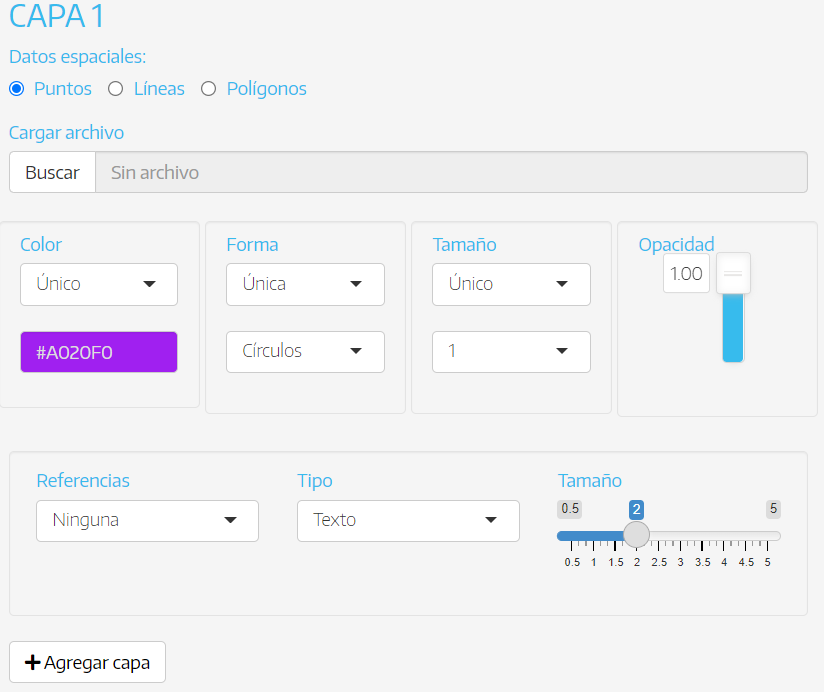
\includegraphics[width=0.8\linewidth,height=0.5\textheight]{imagenes/mapear1}

Al trabajar con datos de estas características se pueden representar
distintas geometrías, así como utilizar diferentes formatos de archivo:

\begin{itemize}
\item
  \textbf{Geometrías}: las principales formas de representación de datos
  espaciales son los \textbf{(i) puntos}, georeferenciados con una
  latitud y longitud (por ejemplo, las coordenadas de un hotel); las
  \textbf{(ii) líneas}, que representan un sucesión de puntos (por
  ejemplo, una ruta); y los \textbf{(iii) polígonos}, que configuran
  áreas (como una provincia).
\item
  \textbf{Formatos}: en el caso de puntos es común utilizar archivos con
  extensión \emph{.xlsx} o \emph{.csv} donde se cuenta con una columna
  para la latitud y otra para la longitud. Para representar líneas y
  polígonos, se suele guardar la información en formatos específicos
  como \emph{.kml} o \emph{.geojson}.
\end{itemize}

Además el archivo debe cumplir con ciertos requisitos, como el formato
en el que están escritas las coordenadas, de manera que la lectura de
los datos sea correcta. En la aplicación se describen estos
requerimientos y se provee de un archivo descargable como modelo para
estructurar los datos.

La interfaz de \textbf{mapeAr} permite al usuario personalizar algunos
parámetros estéticos de las capas cargadas, como por ejemplo, el color y
el tamaño, para que el resultado se ajuste a sus necesidades.

Finalmente, con el botón de descarga se ofrece la posibilidad de
exportar el mapa como imagen en distintos formatos, para poder
compartirlo, utilizarlo en documentos o presentaciones, etc.

\newpage

\hypertarget{referencias}{%
\section*{Referencias}\label{referencias}}
\addcontentsline{toc}{section}{Referencias}

\hypertarget{refs}{}
\begin{CSLReferences}{1}{0}
\leavevmode\hypertarget{ref-shiny}{}%
Chang, Winston, Joe Cheng, JJ Allaire, Carson Sievert, Barret Schloerke,
Yihui Xie, Jeff Allen, Jonathan McPherson, Alan Dipert, and Barbara
Borges. 2021. \emph{Shiny: Web Application Framework for r}.
\url{https://CRAN.R-project.org/package=shiny}.

\leavevmode\hypertarget{ref-ggplot2}{}%
Wickham, Hadley. 2016. \emph{Ggplot2: Elegant Graphics for Data
Analysis}. Springer-Verlag New York.
\url{https://ggplot2.tidyverse.org}.

\end{CSLReferences}




\end{article}
\end{document}
